%------------Ejercicio 1---------------------------------------

\begin{question}
    Sea la función

    \[
        f(x,y) =
        \begin{cases}
            \displaystyle \frac{yx^3-xy^3}{x^2+y^2} & \text{si}\; (x,y) \neq (0,0) \\[10pt]
            \qquad 0                                & \text{si}\; (x,y)=(0,0)
        \end{cases}
    \]

    probar que no existe $\delta>0$ tal que $f$ sea clase $C^2$ en $B_{\delta}(0,0)$.
\end{question}

%------------Ejercicio 2---------------------------------------

\begin{question} Calcular
    \[
        \lim_{(x,y) \to (0,0)}
        \frac{e^{2x}e^{3y} - 1 - 2x -3y - 3x^2 - 6yx - \frac{11}{2}y^2}{x^2+y^2}
    \]
\end{question}

%------------Ejercicio 3---------------------------------------

\begin{question}
    Sea $S$ el conjunto de puntos en  $\Rn{3}$  que forman la esfera de centro $(3,4,5)$ tal que el $(0,0,0) \in S$.
    \begin{itemize}
        \item [a.] Hallar el plano tangente a $S$ en $(0,0,0)$.
        \item [b.] Hallar otro plano que sea tangente a $S$ y paralelo al del ítem a.
    \end{itemize}
\end{question}

%------------Ejercicio 4---------------------------------------

\begin{question}
    Hallar los puntos de $A:(x-1)^2 + (y-1)^2 = 4$ que realicen la distancia mínima y máxima al origen.
\end{question}

\newpage
%-----------Solucion 1--------------------------------------------

\begin{solution}
    Por el teorema de Schwartz sabemos que si $f \in\ C^2$ en  $B_{\delta}(0,0)$
    entonces $$  f_{xy} (x,y) = f_{yx} (x,y) \quad \forall (x,y) \in B_{\delta}(0,0).$$ En particular, deber\'ia pasar que $f_{xy} (0,0) = f_{yx}(0,0).$ Veamos que esto \'ultimo no sucede.

    \begin{equation}
        f_x(x,y) = \frac{(3yx^2-y^3)(x^2+y^2) - (yx^3-xy^3)2x}{(x^2+y^2)^2} \label{eq:partXej1}
    \end{equation}

    \begin{equation}
        f_y(x,y) = \frac{(x^3-3xy^2)(x^2+y^2) - (yx^3-xy^3)2y}{(x^2+y^2)^2}  \label{eq:partYej1}
    \end{equation}

    Para $(x,y) = (0,0)$, calculamos las derivadas por definición.
    \[
        f_x(0,0)  = \lim_{h\to0} \frac{f(h,0) - f(0,0)}{h} = 0
    \]
    \[
        f_y(0,0)  =  \lim_{h\to0} \frac{f(0,h) - f(0,0)}{h} = 0
    \]

    Ya tenemos definidas las derivadas parciales de $f$ en todo $\Rn{2}.$
    \[
        f_x(x,y) =
        \begin{cases}
            \eqref{eq:partXej1} & \text{si}\ (x,y) \neq (0,0) \\
            0                   & \text{c.c.}
        \end{cases}
    \]

    \[
        f_y(x,y) =
        \begin{cases}
            \eqref{eq:partYej1} & \text{si}\ (x,y) \neq (0,0) \\
            0                   & \text{c.c.}
        \end{cases}
    \]

    Ahora podemos calcular las derivadas parciales cruzadas de segundo orden por definición.

    \begin{equation}
        f_{xy}(0,0) = \lim_{h\to0} \frac{f_x(0,h) - f_x(0,0)}{h} \label{eq:limDef1}
    \end{equation}

    \begin{equation}
        f_{yx}(0,0) = \lim_{h\to0} \frac{f_y(h,0) - f_y(0,0)}{h}  \label{eq:limDef2}
    \end{equation}

    Por \eqref{eq:partXej1} y \eqref{eq:partYej1}, se puede observar que
    \[
        f_x(0,h) = -h \text{ y } f_y(h,0) = h.
    \]

    Entonces por \eqref{eq:limDef1} Y \eqref{eq:limDef2}
    \[
        f_{xy}(0,0) = -1 \neq f_{yx}(0,0) = 1.
    \]

    $\therefore\;$ no existe $\delta>0$ tal que $f$ sea clase $C^2$ en $B_{\delta}(0,0)$.
\end{solution}

%-----------Solucion 2--------------------------------------------

\begin{solution}
    Para resolverlo debemos intuir que está conformado por el límite de buena aproximación de un polinomio de Taylor de segundo orden centrado en el origen de una función. Buscamos una expresión para dicho polinomio y para la función.

    Llamemos $f(x,y) = e^{2x}e^{3y}$, notemos que $f$ es de clase $C^3(\Rn{2}).$  Entonces, podemos definir su polinomio de Taylor de segundo orden centrado en el origen, $ P_2(x,y)$, y adem\'as vale el teorema de resto de Taylor
    \[
        P_2(x,y) = f(0,0) + \grad f(0,0)\cdot(x,y) + \frac{1}{2}(x,y)\boldsymbol{H}_f(0,0)(x,y)^\mathrm{T},
    \]
    siendo $\boldsymbol{H}_f(0,0)$ la matriz hessiana de $f$ evaluada en el origen.

    Tenemos que
    \begin{gather*}
        f(0,0) = 1,\\[.2cm]
        \grad f(x,y) = \left(2e^{2x}e^{3y}, 3e^{2x}e^{3y}\right) \implies \grad f(0,0) = (2,3),\\[.25cm]
        \boldsymbol{H}_f(x,y) = \left(\begin{array}{cc}
                4e^{2x}e^{3y} & 6e^{2x}e^{3y} \\[10pt]
                6e^{2x}e^{3y} & 9e^{2x}e^{3y}
            \end{array}\right) \implies \boldsymbol{H}_f(0,0) = \left(\begin{array}{cc}
                4 & 6 \\
                6 & 9
            \end{array}\right).
    \end{gather*}
    Entonces queda
    \[
        \begin{aligned}
            P_2(x,y)      & = 1+(2,3)\cdot(x,y)+\frac{1}{2}(x,y)
            \left(\begin{array}{cc}  
                    4 & 6 \\
                    6 & 9
                \end{array}\right)
            \left(\begin{array}{cc}
                          x \\
                          y
                      \end{array}\right)                                                     \\[4pt]
            \iff P_2(x,y) & = 1 + 2x + 3y + 2x^2 + 6xy + \frac{9}{2}y^2.
        \end{aligned}
    \]
    Expresamos el error como
    \[
        R_2(x,y) = f(x,y) - P_2(x,y).
    \]
    Por tanto, podemos reescribir el límite original como
    \[\\[2pt]
        \lim_{(x,y) \to (0,0)} \frac{R_2(x,y) - x^2 - y^2}{\|(x,y)\|^2} =
        \lim_{(x,y) \to (0,0)} \left( \frac{R_2(x,y)}{\|(x,y)\|^2} - \frac{x^2+y^2}{\|(x,y)\|^2} \right) = -1,
    \]
    pues el primer término tiende a 0 por el teorema de Taylor  y el segundo  tiende claramente a $1.$
\end{solution}

%-----------Solucion 3--------------------------------------------

\begin{solution}
    a. Dado que el origen pertenece a $S$ y conocemos su centro, podemos hallar la ecuación de la esfera.
    \[
        S:(x-3)^2 + (y-4)^2 + (z-5)^2 = 50
    \]
    \begin{center}
        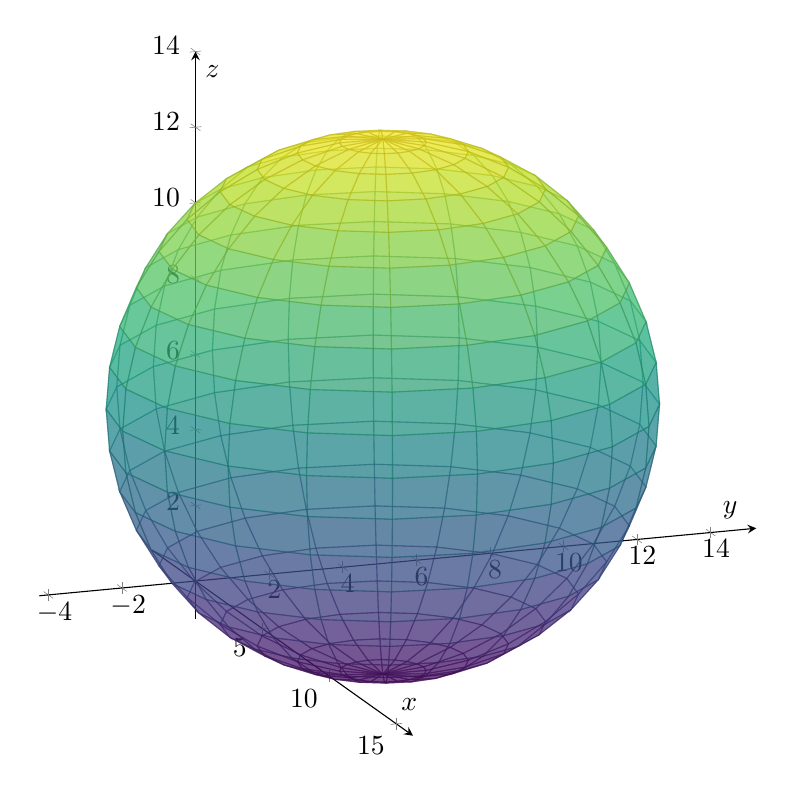
\begin{tikzpicture}
            \begin{axis}[
                    view={70}{15},
                    axis equal,
                    width=14cm,
                    height=12cm,
                    axis lines = center,
                    xlabel = {$x$},
                    ylabel = {$y$},
                    zlabel = {$z$},
                    zmin=-1,
                    xmin=-1,
                    ymin=-1,
                    zmax=14,
                    xmax=14,
                    ymax=12,
                    colormap/viridis
                    % ticks=none,
                ]
                \addplot3[
                    surf,
                    opacity=0.5,
                    samples=21,
                    domain=0:360,
                    y domain=0:180,
                    z buffer=sort
                ]
                ({3 + sqrt(50) * sin(y) * cos(x)},
                {4 + sqrt(50) * sin(y) * sin(x)},
                {5 + sqrt(50) * cos(y)});

            \end{axis}
        \end{tikzpicture}
    \end{center}

    Llamando $$f:\mathbb{R}^3 \rightarrow \mathbb{R}:  f(x,y,z) = (x-3)^2 + (y-4)^2 + (z-5)^2 - 50$$
    tenemos que $$S=C(f,0). $$
    Buscamos el plano $\Pi$, tangente a $C(f,0)$ y que pase por $(0,0,0)$. Sabemos que la ecuación de  $\Pi$  es  de la forma
    \[
        \Pi:\grad f(0,0,0) \cdot (x-0,y-0,z-0) = 0.
    \]
    Es f\'acil ver que $\grad f(0,0,0) = (-6,-8,-10).$  Luego, una posible ecuaci\'on es
    \[\\[1pt]
        \Pi: 3x + 4y + 5y = 0.
    \]

    b. Dado que el único plano paralelo a otro tangente a un punto en una esfera es el que se encuentra en el polo opuesto de ésta, buscamos el plano tangente $\Pi'$ a ese otro punto $\mathbf{w}$. Llamando $\mathbf{v} = (-3,-4,-5)$ al vector que sale del centro de la esfera y termina en el origen, queda que
    \[
        \mathbf{w} = (3,4,5) - \mathbf{v} = (6,8,10).
    \]
    Como $\Pi$ y $\Pi'$ son paralelos, su vector normal $\textbf{n}$ es el mismo.
    \[
        \begin{aligned}
            \implies & \Pi ': \textbf{n} \cdot ((x,y,z) - \mathbf{w}) = 0 \\
            \iff     & \Pi ': 3(x-6) + 4(y-8) + 5(z-10) = 0               \\
            \iff     & \Pi ':3x + 4y + 5y = 100
        \end{aligned}
    \]

    \begin{center}
        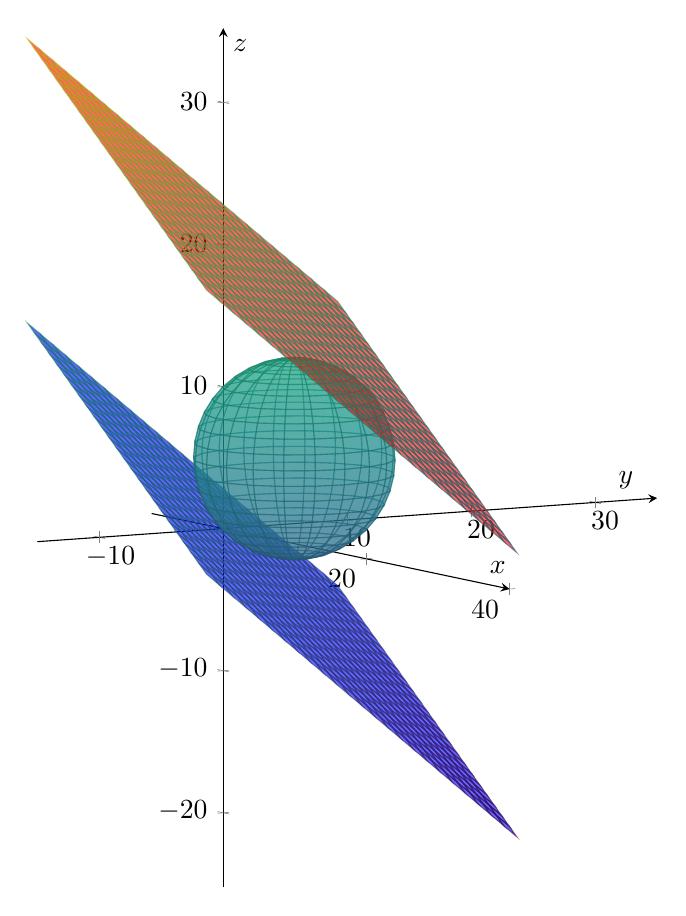
\begin{tikzpicture}
            \begin{axis}[
                    view={60}{7},
                    axis equal,
                    width=14cm,
                    height=14cm,
                    axis lines = center,
                    xlabel = {$x$},
                    ylabel = {$y$},
                    zlabel = {$z$},
                    zmin=-20,
                    xmin=-10,
                    ymin=-10,
                    zmax=30,
                    xmax=40,
                    ymax=30,
                    colormap/viridis
                ]

                % Add the second plane
                \addplot3[
                    surf,
                    fill = blue,
                    opacity=0.6,
                    domain=-10:15,
                    y domain=-10:15,
                ]
                {- (3*x + 4*y)/5}; % Equation of the second plane: 3x + 4y + 5z = 0

                \addplot3[
                    surf,
                    opacity=0.5,
                    samples=21,
                    domain=0:360,
                    y domain=0:180,
                    z buffer=sort
                ]
                ({3 + sqrt(50) * sin(y) * cos(x)},
                {4 + sqrt(50) * sin(y) * sin(x)},
                {5 + sqrt(50) * cos(y)});

                % Add the first plane
                \addplot3[
                    surf,
                    fill = red,
                    opacity=0.6,
                    domain=-10:15,
                    y domain=-10:15,
                ]
                {20-(3*x + 4*y)/5}; % Equation of the first plane: 3x + 4y + 5z = 100

            \end{axis}
        \end{tikzpicture}
    \end{center}
\end{solution}


\vspace{0.3 cm}

%-----------Solucion 4--------------------------------------------

\begin{solution}
    Sean
    \[
        f: \mathbb{R}^2 \rightarrow \mathbb{R}, \; f(x,y) = \text{dist}^2\Big((x,y);(0,0)\Big)  = x^2 + y^2
    \]
    y
    \[
        g: \mathbb{R}^2 \rightarrow \mathbb{R}, \; g(x,y) = (x-1)^2 + (y-1)^2 - 4,
    \]
    luego $A=C(g,0) $.

    Como $f,g \in C^1( \mathbb{R}^1),$  el teorema de los multiplicadores de Lagrange nos dice que si $f \big\rvert _A$ tiene un extremo local en un punto \textbf{x} entonces necesariamente los vectores $\grad f(\textbf{x})$ y $\grad g(\textbf{x})$ son paralelos si $\grad g(\textbf{x}) \neq 0$.   Además como $f$ es continua sobre el conjunto $A$ que es cerrado y acotado, por el teorema de Weierstrass, sabemos que $f$ alcanza m\'aximo y m\'inimo en $A$. Luego planteamos el siguiente sistema de ecuaciones
    \[
        \grad f(x,y) = \lambda \grad g(x,y), \; \lambda \in \mathbb{R}, \; (x,y) \in A \\
        \iff \begin{cases}
            2x = 2\lambda(x-1) \\
            2y = 2\lambda(y-1) \\
            (x-1)^2 + (y-1)^2 = 4
        \end{cases}
    \]
    Resolviendo el sistema queda $x=y$  \;  y \[ \begin{cases}
            x=   x_1=1+\sqrt{2} \\
            x=  x_2=1-\sqrt{2}.
        \end{cases}\]
    $\implies (x_1,x_1)$  y $(x_2,x_2)$  son ambos extremos absulutos de la función $f$  en $A$. Como $f(x_1,x_1) > f(x_2,x_2) \implies (x_1,x_1)$ es máximo absoluto y $(x_2,x_2)$ es mínimo absoluto.

    Luego  la distancia mínima del circulo al origen es $\sqrt{f(x_2,x_2)} = 2-\sqrt{2} $ y la distancia máxima $\sqrt{f(x_1,x_1)} = 2+\sqrt{2}$.
\end{solution}

